%% Direttive TeXworks:
% !TeX root = ../maltoni_niccolo_tesi.tex
% !TEX encoding = UTF-8 Unicode
% !TEX program = arara
% !TEX TS-program = arara
% !TeX spellcheck = it-IT

%% Direttive Arara:
% arara: pdflatex: { shell: yes, synctex: yes, action: batchmode, options: "-halt-on-error -file-line-error-style" }
% arara: frontespizio
% arara: biber
% arara: pdflatex: { shell: yes, synctex: yes, action: batchmode, options: "-halt-on-error -file-line-error-style" }
% arara: pdflatex: { shell: yes, synctex: yes, action: nonstopmode, options: "-halt-on-error -file-line-error-style" }

\chapter{Contributo}\label{ch:contributo}
    In questo capitolo verrà analizzato il contributo fornito al progetto, elencando i requisiti necessari e analizzando il processo di soddisfazione degli stessi.

    L'obiettivo principale è quello di integrare una nuova interfaccia per la simulazione, al fine di semplificare l’adozione del simulatore da parte di utenti inesperti.

    \section{Analisi dei requisiti}\label{sec:analisi}
        Lo studio del lavoro illustrato in questa tesi ha inizio con l'analisi dei requisiti dell’interfaccia utente, ossia cosa l'applicazione deve mostrare a schermo.

        Questa sezione si occuperà di enunciare i requisiti funzionali e non funzionali individuati.

        \subsection{Requisiti funzionali}\label{sub:funzionali}
            I requisiti funzionali (\figurename~\ref{fig:useCase}) descrivono il comportamento che il sistema deve avere:
            descrivono le funzionalità del sistema software, in termini di servizi che il sistema software deve fornire, di come il sistema software reagisce a specifici tipi di input e di come si comporta in situazioni particolari.

            \subsubsection{Rappresentazione dell'ambiente di simulazione}\label{subsub:seeEnv}
                Essendo la componente grafica da reimplementare quella legata alla simulazione in escuzione, requisito fondamentale è che la GUI possa rappresentare l'ambiente con le maggiori possibilità di dettaglio possibile.

                Di conseguenza, deve essere presente uno spazio disegnabile in cui si possa avere una rappresentazione grafica di quanto accade, ma anche contatori che mostrino l'avanzamento della simulazione in termini di tempo (secondi) trascorso e passaggi (\engEmph{step}) effettuati.

            \subsubsection{Gestione degli effetti}\label{subusub:manageEffects}
                La nuova interfaccia deve rendere possibile all'utente di poter aggiungere nuovi effetti allo \engEmph{stack} di rappresentazione e modificarne le proprietà a tempo di esecuzione.

                Inoltre attraverso la GUI l'utente deve poter salvare lo stack di effetti presente in quel momento e caricarlo in un secondo momento, mantenendo tutte le proprietà definite manualmente.

                Infine, deve essere possibile nascondere singoli effetti o gruppi di essi senza rimuoverli dallo \engEmph{stack}.

            \subsubsection{Effetti standard per nodi e collegamenti}\label{subusub:defaultEffects}
                Devono essere implementati effetti adibiti alla rappresentazione dei singoli nodi come punti e dei collegamenti tra i nodi di un vicinato.

                Questi effetti dovranno essere caricati automaticamente al lancio dell'applicazione, salvo diversamente specificato.

            \subsubsection{Interazione con simulazione e ambiente rappresentato}\label{subsub:interazione}
                L'interfaccia deve mettere a disposizione dell'utente la capacità di interagire con la simulazione, potendo fermarla e riavviarla, interagire con i nodi e spostarsi tra essi. Deve essere possibile effettuare pan e zoom sull'ambiente rappresentato.

                Le possibilità di interazione non devono essere vincolate al puntatore del mouse, ma deve supportare anche le scorciatoie da tastiera.

            \subsubsection{Rappresentazione di ambienti con mappa}\label{subsub:mappa}
                Deve essere fornito il supporto alle mappe come sfondo degli ambienti nella rappresentazione di simulazioni che coinvolgano questo aspetto.

                \begin{figure}[htbp]
                    \centering
                    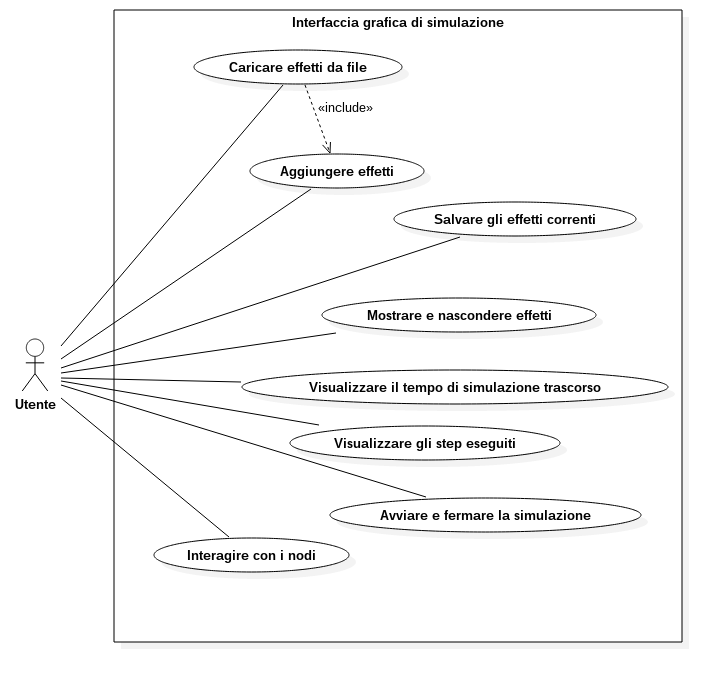
\includegraphics[scale=0.55]{img/useCase}
                    \caption{Requisiti funzionali principali}
                    \label{fig:useCase}
                \end{figure}

        \subsection{Requisiti non funzionali}\label{sub:nonFunzionali}
            I requisiti non funzionali descrivono le proprietà non comportamentali che il sistema deve possedere, come efficienza, affidabilità, sicurezza, performance, ma anche caratteristiche del processo di sviluppo e caratteristiche esterne.

            \subsubsection{JavaFX}\label{subsub:jfx}
                Come specificato nella sezione~\vref{sec:motivi}, il processo di sviluppo deve coinvolgere la libreria JavaFX come framework per la costruzione dell'interfaccia.

            \subsubsection{Performance}\label{subsub:performance}
                L'interfaccia grafica deve quanto più possibile non gravare sulle prestazioni del motore di simulazione; in particolare, poiché JavaFX non è nativamente \engEmph{thread-safe}, è necessario gestire la concorrenza in modo oculato.

            \subsubsection{Supporto Hi-DPI}\label{subsub:hidpi}
                L'interfaccia non deve perdere di usabilità e qualità di rappresentazione su alcun tipo di schermo, indipendentemente dalla risoluzione e dalla densità di pixel.Per fare questo si devono quindi utilizzare quanto più possibile grandezze relative e sfruttare al meglio in tal senso le funzionalità offerte da JavaFX.

            \subsubsection{Serializzazione \engEmph{Human-readable}}
                Deve essere possibile serializzare gli effetti in un formato testo, in modo tale che possa essere facilmente creato e/o modificato manualmente in modo semplice, senza coinvolgere necessariamente l'interfaccia di Alchemist.

    \section{Fonti d'ispirazione}\label{sec:ispirazione}
        Una volta chiariti i requisiti dell'interfaccia, il passo successivo riguarda la progettazione dell'interfaccia.

        Per poter disegnare dei mockup da utilizzare come bozzetti, sono state fatte ricerche in merito alle interfacce grafiche utilizzate da altri simulatori, anche a scopo non strettamente scientifico.

        Infine, si è scelto tra i design moderni più comuni e apprezzati uno da adottare per fornire un aspetto grafico a cui l'utente medio fosse già abituato e che potesse fornire un'esperienza di utilizzo più gradevole.

        \subsection{Simulatori a scopo videoludico}\label{sub:videogame}
            Come già segnalato nelle sezioni precedenti, è importante che l'interfaccia grafica si presenti semplice e immediata anche per l'utente non avanzato. Di conseguenza, si è scelto di analizzare con più attenzione le GUI di simulatori sviluppati a scopo prettamente videoludico, in quanto più orientati all'immediatezza d'uso rispetto ai simulatori di concezione scientifica.

            Tra i videogiochi di simulazione più famosi, è stato interessante analizzare SimCity, il quale all'epoca del lancio fu molto apprezzato~\cite{friedman1995} appunto per il gameplay e l'interfaccia piuttosto innovativi, e i giochi della serie Universe Sandbox del team Giant Army.

            \subsubsection{SimCity}\label{subsub:simcity}
                La celebre serie di videogiochi di simulazione SimCity~\cite{simcity}, ideata da Will Wright tra gli anni `80 e gli anni `90 ispirandosi alla ricerca contenuta nel saggio di architettura \engEmph{A pattern language}~\cite{wiredWright, aPatternLanguage}, sviluppata da Maxis e distribuita da Electronics Arts, è tutt'ora considerata una delle più innovative per quanto riguarda la storia dei videogiochi di simulazione.

                \begin{figure}[htbp]
                    \centering
                    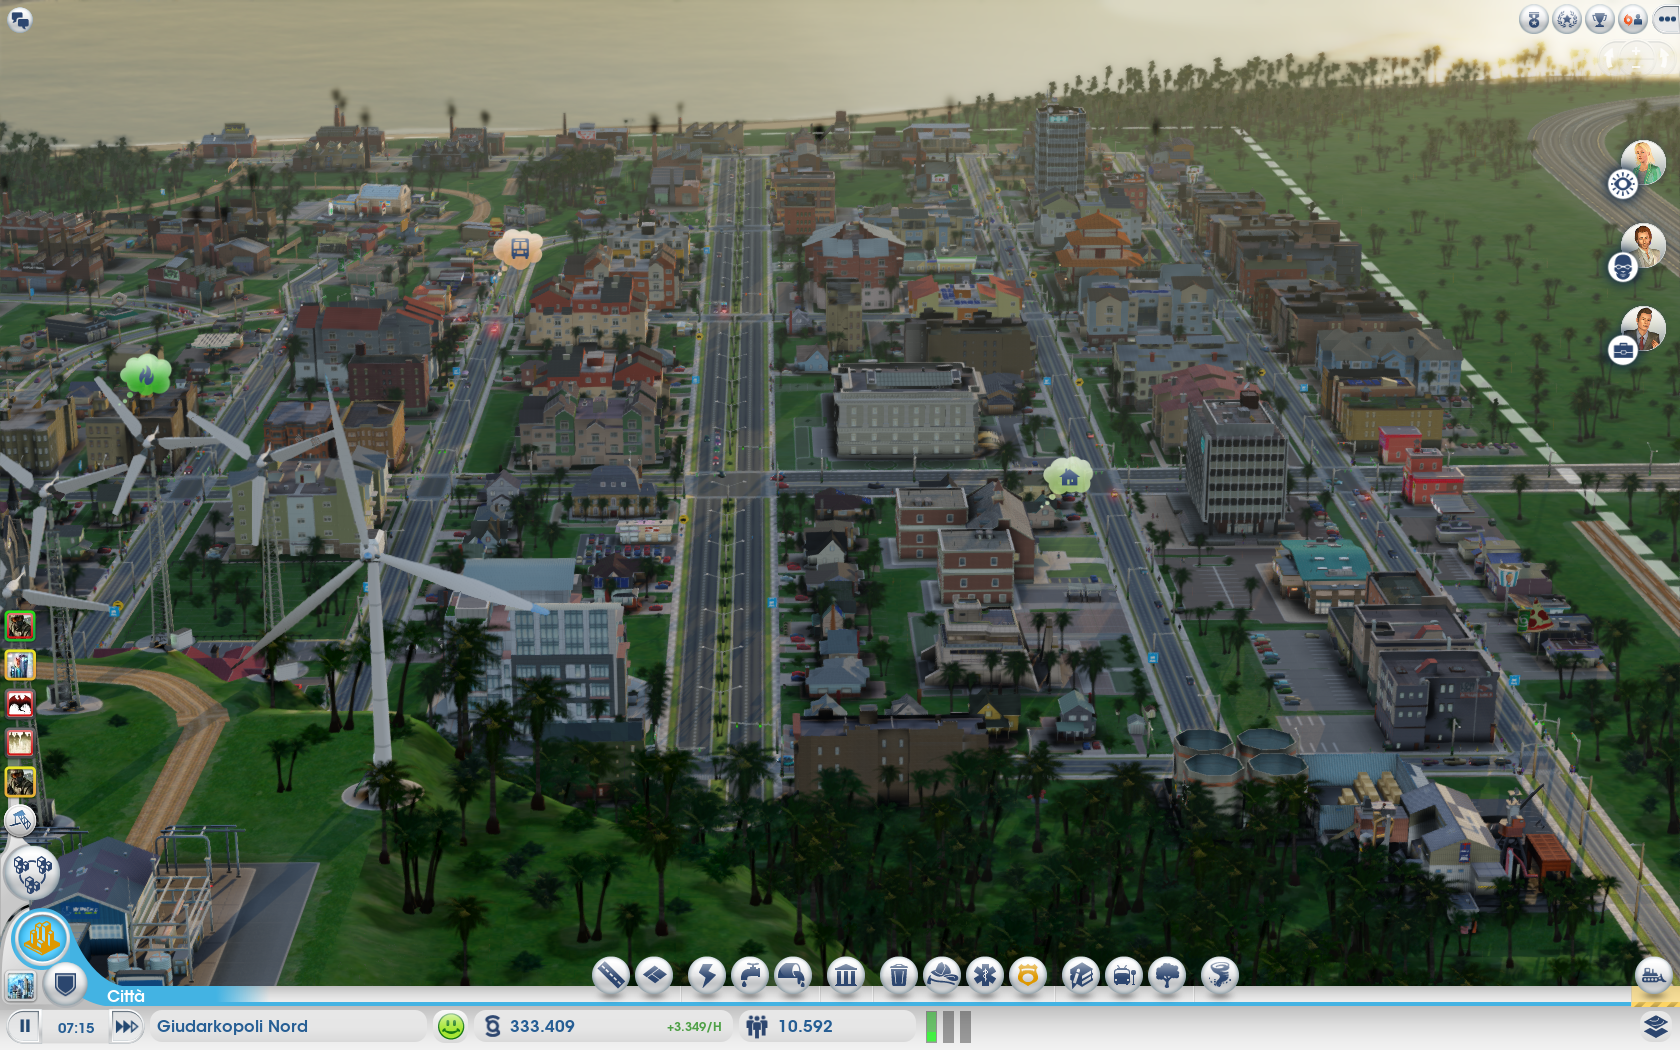
\includegraphics[scale=0.2]{img/SimCity}
                    \caption{SimCity (2013), sviluppato da Maxis e distribuito da EA, tutti i diritti riservati ai ripettivi proprietari}
                    \label{fig:simcity}
                \end{figure}

                % TODO potrebbe essere utile inserire ulteriori dettagli?

            \subsubsection{Universe Sandbox}\label{subsub:universesandbox}
                Altra serie di videogiochi simulativi analizzata è Universe Sandbox.
                Dopo oltre 15 anni di sviluppo~\cite{unisandTechradar}, il primo capitolo~\cite{universeSandboxDixon} è stato rilasciato dallo sviluppatore e artista Dan Dixon nel 2008.
                Il responso positivo lo ha portato a continurare lo sviluppo, tanto da fondare la compagnia Giant Army~\cite{universeSandboxGiantArmy}, che ha rilasciato nel 2015 la seconda iterazione della saga, Universe Sandbox\ap{2}~\cite{universeSandbox2}.

                % TODO approfondire analisi ?

                Per il design dell'interfaccia, è stato proprio il secondo capitolo a fungere da maggior fonte d'ispirazione. Essa va a riprendere la classica interfaccia utilizzata da videogiochi simulativi come il già citato SimCity (\figurename~\ref{fig:simcity}), ma andando a rimuovere buona parte degli ornamenti grafici tipici delle GUI a scopo videoludico, andando a preferire uno stile molto più pulito e semplificato; il sistema di interazione a sviluppo verticale e a popup viene sostituito con uno sviluppo orizzontale di pannelli (definito \emph{Modello multi-paned}~\cite{multipanedmodel}) che vanno a raccogliere tutte le impostazioni e i parametri.

                La simulazione viene rappresentata sullo sfondo, come in SimCity, ma con effetti di trasparenza non presenti nel gioco di EA.

                % TODO approfondire analisi ?

                \begin{figure}[htbp]
                    \centering
                    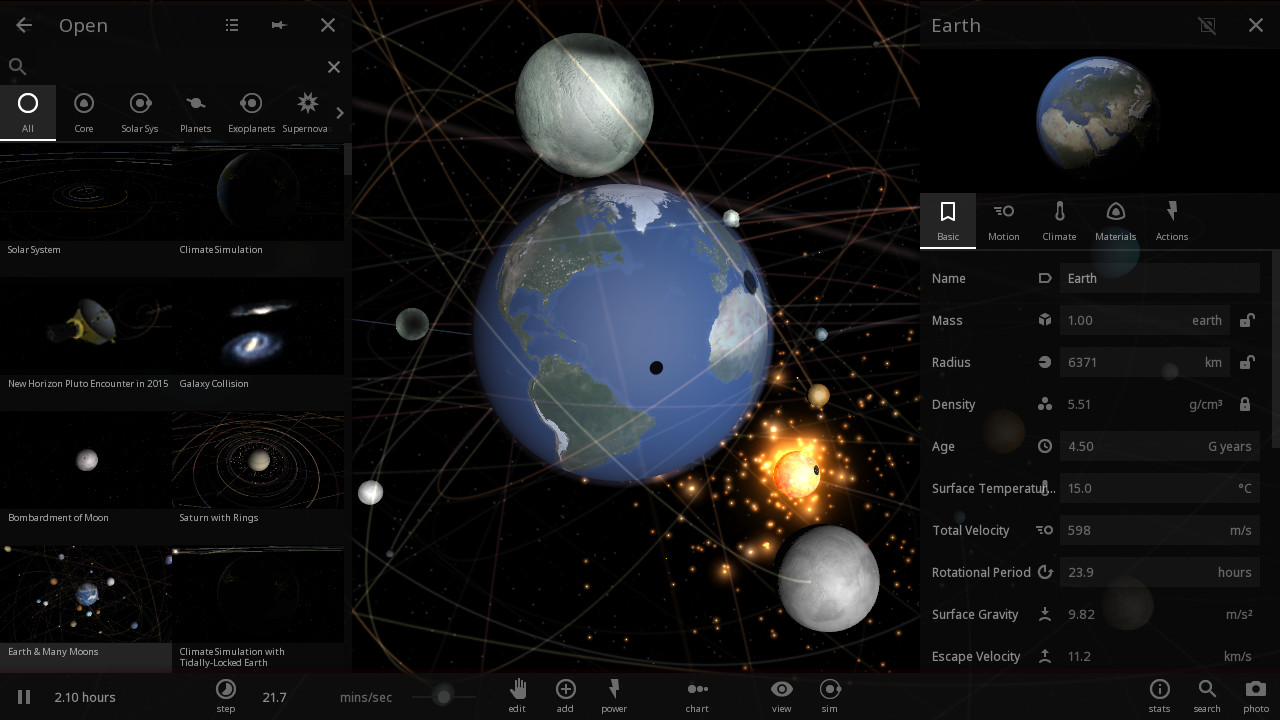
\includegraphics[scale=0.35]{img/universesandboxpanels}
                    \caption{Universe Sandbox\ap{2} (2015), sviluppato e distribuito da Giant Army, tutti i diritti riservati ai ripettivi proprietari}
                    \label{fig:universesandboxpanels}
                \end{figure}

        \subsection{Material Design}\label{sub:material}
            Uno dei maggiori motivi che hanno portato l'interfaccia grafica di Alchemist a necessitare di un rinnovamento è stata l'intenzione di semplificarla all'occhio dell'utente non esperto, fornendo un'esperienza completa e gradevole.
            Era dunque necessario scegliere uno stile grafico familiare, moderno e facilmente adattabile a quella che sarebbe essere la nuova interfaccia che si stava progettando.

            Prendendo come base l'interfaccia di Universe Sandbox illustrata nella sezione~\ref{subsub:universesandbox}, è possibile notare che il design di base sia estremamente ``flat''; si è deciso di valutare i possibili design a cui adeguare la UX che si aveva intenzione di progettare.

            La scelta è infine ricaduta sul Material Design~\cite{material} sviluppato da Google: dal suo annuncio nel giugno del 2014 alla conferenza del Google I/O~\cite{pichai2014google} esso è stato almeno parzialmente adottatto in molte applicazioni web, mobile e desktop, e ben si si presta all'implementazione di un'interfaccia semplice e minimale.

            Si è deciso di utilizzare le icone\footnote{\url{https://material.io/icons/}} e le direttive in merito a dimensioni e palette di colore\footnote{\url{https://material.io/color/}} fornite da Google.

    \section{Design dell'interfaccia}\label{sec:design}
        Una volta chiariti i requisiti e le possibili fonti di ispirazione per la struttura della GUI da realizzare, sono stati disegnati dei mockup che potessero rappresentare una linea guida per l'implementazione concreta dell'interfaccia.

        \begin{figure}[htbp]
            \centering
            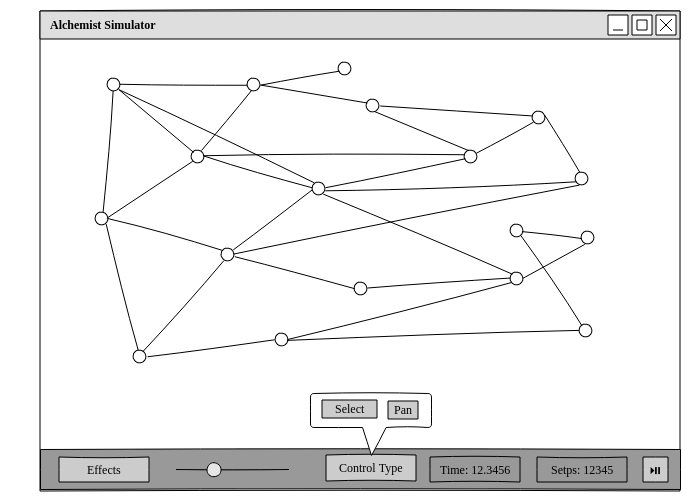
\includegraphics[scale=0.4]{img/withNodes/main_window}
            \caption{Mockup dell'interfaccia principale}
            \label{fig:mock:mainWindow}
        \end{figure}

        Come è possibile vedere dalla \figurename~\vref{fig:mock:mainWindow}, si è scelto di adottare un'interfaccia composta da uno spazio disegnabile centrale, al quale viene sovrapposta nella parte inferiore una barra contenente dei controlli che permettono un'interazione semplice e diretta con le funzionalità di base:

        \begin{description}
          \item [Play/Pausa] Partendo da destra, è presente un bottone che permette di avviare e mettere in pausa la simulazione.

          Esso funge anche da indicatore per lo stato attuale della simulazione: qualora essa venga avviata o fermata da terminale o tramite una scorciatoia da tastiera, l'icona rappresentata sul bottone viene aggiornata per adeguarsi al nuovo stato.

          \item[Avanzamento in termini di tempo e step] Continuando verso sinistra, si trovano spazi dedicati al numero di secondi di simulazione rappresentati e di step effettuati; essi vengono aggiornati durante tutto l'avanzamento del motore di simulazione.

          \item[Gestione del sistema di controllo] Poiché l'interazione tramite mouse deve permettere sia di spostarsi nell'ambiente che selezionare i nodi e interagirvi, è presente un bottone che apre un pannello che permette di scegliere tra spostamento (\engEmph{pan}) e selezione.

          \item[Gestione della velocità] Una barra a scorrimento permette di regolare la velocità di rappresentazione della simulazione.

          \item[Gesione degli effetti] Un bottone sul lato sinistro della barra permette di aprire un pannello sul medesimo lato della finestra per poter controllare gli effetti con i quali rappresentare cosa sta avvenendo nella simulazione.

          Nelle Figure~\vrefrange{fig:mock:groups}{fig:mock:properties} è possibile osservare i diversi livelli del drawer laterale degli effetti.

          \begin{figure}[htbp]
              \centering%
              \subfigure[%
                  Vista dei singoli gruppi di effetti che compongono lo \engEmph{stack}%
                  \label{fig:mock:groups}
              ]{%
                  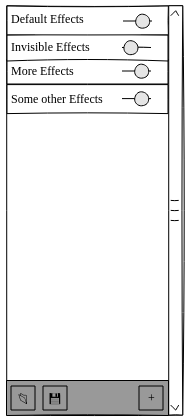
\includegraphics[scale=0.5]{img/cropped/effectgroups_bar_open}
              }%
              \qquad{\LARGE$\Rightarrow$}\qquad
              \subfigure[%
                  Vista dei singoli effetti di un gruppo%
                  \label{fig:mock:effects}%
              ]{%
                  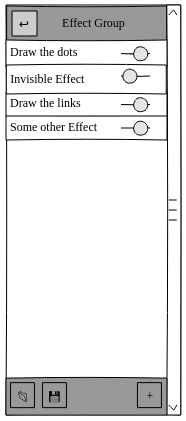
\includegraphics[scale=0.5]{img/cropped/effects_bar_open}
              }%
              \qquad{\LARGE$\Rightarrow$}\qquad
              \subfigure[%
                  Vista delle proprietà di un effetto%
                  \label{fig:mock:properties}%
              ]{%
                  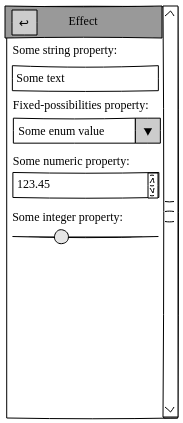
\includegraphics[scale=0.5]{img/cropped/effect_properties_open}
              }
              \caption{Vista del pannello laterale degli effetti nei diversi livelli\label{fig:mock:allEffects}}
          \end{figure}

          % TODO sistema altezza frecce

        \end{description}

    \section{Progettazione}\label{sec:progettazione}
        \subsection{La barra inferiore}\label{sub:barra}
        \subsection{La struttura a drawer}\label{sub:drawer}
        \subsection{L'architettura degli effetti}\label{sub:effetti}
            % \subsubsection{I gruppi di effetti e l'interfaccia \texttt{EffectGroup}}\label{subsub:effectGroup}
            % \subsubsection{I singoli effetti e l'interfaccia \texttt{EffectFX}}\label{subsub:effectFX}
            % \subsubsection{Caricamento, salvataggio e modifica di gruppi di effetti}\label{subsub:serializzazione}
    \section{Dettagli implementativi}\label{sec:dettagli}
        % \subsection{Librerie utilizzate}\label{sub:lib}
        % \subsection{Gestione della concorrenza}\label{sub:concorrenza}
